\chapter{Evaluation der Ergebnisse}\label{evaluation}

Im Folgenden werden die entwickelten Modelle untersucht und evaluiert. Für die beiden \acl{RF}s wird die Implementierung von \texttt{sklearn} genutzt, für die Gradient Boosted Trees die Bibliothek \texttt{XGBoost}, da das \ac{XGB} besser ist als die in \texttt{sklearn}.\footcite[Kapitel 10]{Harrison2019} Die Ergebnisse der Modelle werden sowohl für das reduzierte als auch das vollständige Merkmalsset berechnet, verglichen und aufbauend darauf die Merkmalsauswahl optimiert. Außerdem wird der Einfluss der gewählten Segmentlänge und des gewählten Schwellwertes der Annotation untersucht. Für alle Untersuchungen wird das gleiche Testset wie in Kapitel \ref{analyse} verwendet.

\section{Merkmalsbezogene Modellevaluation} %TODO: besserer Titel? Merkmalsauswahl?

Zunächst werden alle Modelle sowohl mit dem vollständigen Merkmalsset als auch dem reduzierten Merkmalsset verglichen, siehe Tabelle \ref{fig:comparison-all}. Die Ergebnisse der Klassifikation mit Gradient Boosted Trees und \acl{RF}s sind zunächst ähnlich. Bei der Regression erreichen Gradient Bossted Trees eine sehr hohe Coverage von, bei Verwendung aller Merkmale, 80\,\% mit einem zu den anderen Modellen verhältnismäßig hohen \ac{MAE} von 16,04\,\si{FE}. Insgesamt zeigt sich bereits, dass eine deutlich höhere Coverage als bei der reinen Betrachtung der Intervallschätzer des CLIE-Algorithmus erreicht wird. Diese lag beispielsweise für $q\textsubscript{th} = 0.3$ bei 20,93\,\% mit einem \ac{MAE} von 13,90\,\si{FE}.

	\begin{table}[H]
		\begin{tabular}{l | l | l|| c | c | c | c }
 						& Merkmalsset	& Modell			& \ac{MAE} [FE]	& Coverage [\%]	& F1-Score	& AUC	\\ \hline
 		\multicolumn{3}{l ||}{insgesamt}					& 21{,}85		& -				& - 		& -		\\
 		\multicolumn{3}{l ||}{annotiert}					& 3{,}28			& 43{,}21		& - 		& -		\\ \hline
 		\multirow{4}{*}{Klassifikation}
 						& \multirow{2}{*}{reduziert}		
 										& \acs{RF} 		& 13{,}87		& 32{,}09		& 0{,}54	& 0,69	\\
 						&				& \acs{XGB}	& 14{,}60		& 38,10			& 0{,}56	& 0,68	\\\cline{2-7} %TODO: update numbers
 						& \multirow{2}{*}{alle}
 									 	& \acs{RF}		& 12{,}11		& 36,81			& 0{,}61	& 0,75	\\
 						&				& \acs{XGB} 	& 11,38			& 35,93			& 0,62		& 0,75\\\hline
 		\multirow{4}{*}{Regression}
 						& \multirow{2}{*}{reduziert}
 										& \acs{RF}		& 14,34			& 41,21			& 0,57		& 0,69	\\
 						&				& \acs{XGB}	& 12{,}63		& 23{,}12		& 0{,}44	& 0,65	\\\cline{2-7} % TODO update numbers		
 					 	& \multirow{2}{*}{alle}		
 					 					& \acs{RF}		& 12,56			& 46,27			& 0,64		& 0,75\\
 					 	&				& \acs{XGB} & 16,04			& 81,80			& 0,65		& 0,74\\
		\end{tabular}
		\caption{Vergleich der aller Modelle mit reduziertem und vollständigem Merkmalsset}
		\label{fig:comparison-all}
	\end{table}

Des Weiteren zeigt sich, dass das reduzierte Merkmalsset entgegen der Erwartungen zu etwas schlechteren Ergebnissen führt. Eine Betrachtung der Wichtigkeit der Merkmale für die Modelle mit vollständigem Merkmalsset zeigt, dass für das vollständige Merkmalsset jeweils $\text{ratio}\textsubscript{acf}$ und $\text{ratio}\textsubscript{acf}$ zu den wichtigsten Merkmalen gehören, die beide aussortiert wurden. In Abbildung \ref{fig:rf-clf-all-importances} ist die Verteilung der Relevanz der Merkmale gezeigt. Ein Test mit einem \ac{RF}-Klassifikator mit dem reduzierten Merkmalsset zuzüglich den oben genannten Merkmalen zeigt, dass sich die Performance im Vergleich zum vollständigen Merkmalsset so sogar minimal verbessert und eine \ac{MAE} von 12,01\,\si{FE} bei einer Coverage von 37,05\,\% erreicht.
\begin{figure}[h]
	\centering
	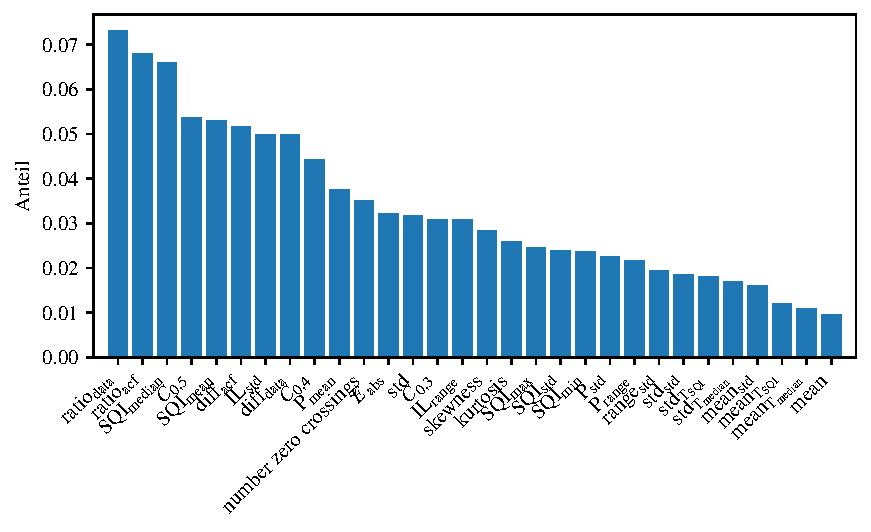
\includegraphics{pic/rf-clf-all-importances.pdf}
 	\caption{Wichtigkeit der Merkmale des \ac{RF}-Klassifikators mit vollständigem Merkmalsset}
 	\label{fig:rf-clf-all-importances}
\end{figure}

Bei den folgenden Untersuchungen wird deshalb das erweiterte reduzierte Merkmalsset verwendet, dass die folgenden Merkmale enthält:
\begin{multicols}{2}
\begin{itemize}
	\item Mittelwert
	\item Kurtosis
	\item Schiefe
	\item $\text{diff}\textsubscript{acf}$
	\item $\text{diff}\textsubscript{data}$
	\item $\text{ratio}\textsubscript{acf}$
	\item $\text{ratio}\textsubscript{data}$
	\item $\text{SQI}\textsubscript{std}$
	\item $\text{SQI}\textsubscript{min}$
	\item $\text{SQI}\textsubscript{median}$
	\item $\text{P}\textsubscript{range}$
	\item $\text{P}\textsubscript{mean}$
	\item $\text{mean}\textsubscript{T\textsubscript{median}}$
	\item $\text{std}\textsubscript{T\textsubscript{median}}$
	\item $\text{mean}\textsubscript{T\textsubscript{SQI}}$
	\item $\text{std}\textsubscript{T\textsubscript{SQI}}$
	\item $\text{IL}\textsubscript{std}$
	\item $\text{mean}\textsubscript{std}$
	\item $C_{0,5}$
	\item $C_{0,4}$
	\item $C_{0,3}$
\end{itemize}
\end{multicols}

Eine weitere Merkmalsreduktion mit rekursiver Merkmals

	
Betrachtet man die Wichtigkeit der Merkmale der beiden Klassifikationsmodelle, fällt auch, dass bei dem Gradient Boosted Trees Klassifikator ein Merkmal allein deutlich wichtiger als alle anderen ist, sowohl beim reduzierten als auch beim vollständigen Merkmalsset. Bei den \ac{RF}-Modellen dagegen, ist die Wichtigkeit gleichmäßiger verteilt. Der direkte Vergleich ist in Abbildung \ref{fig:importances-comparison-rf-xgb-clf} zu sehen. Trotz der unterschiedlichen Gewichtung der Merkmale erzielen beide Modelle ähnliche Ergebnisse. Allerdings ist der \ac{XGB}-Klassifikator weniger stabil für Verzerrung in dem mit Abstand wichtigstem Merkmal $C_{0.5}$.

 \begin{figure}[h]
 	\centering
		\begin{subfigure}{.495\textwidth}
			\centering
 			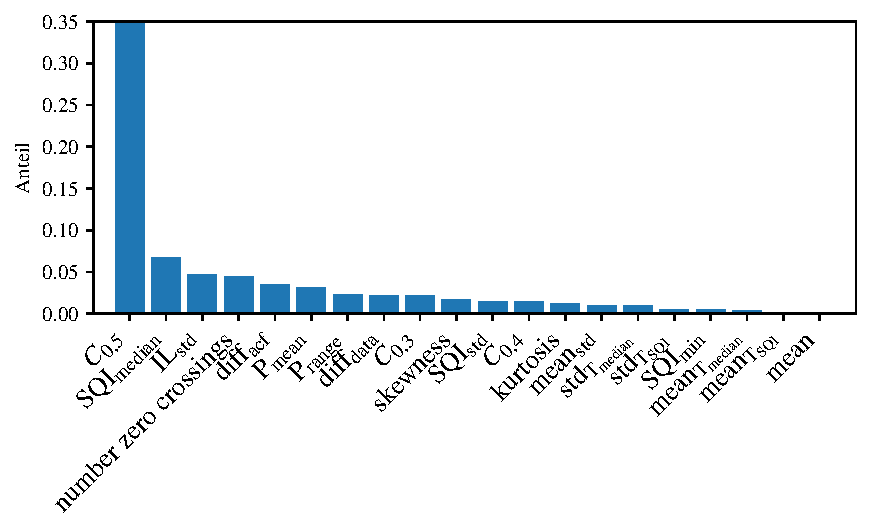
\includegraphics[width=\textwidth]{pic/xgb-clf-reduced-importances.pdf}
 			\caption{\ac{XGB}-Klassifikator}
 		\end{subfigure}
    	\begin{subfigure}{.495\textwidth}
    		\centering
 			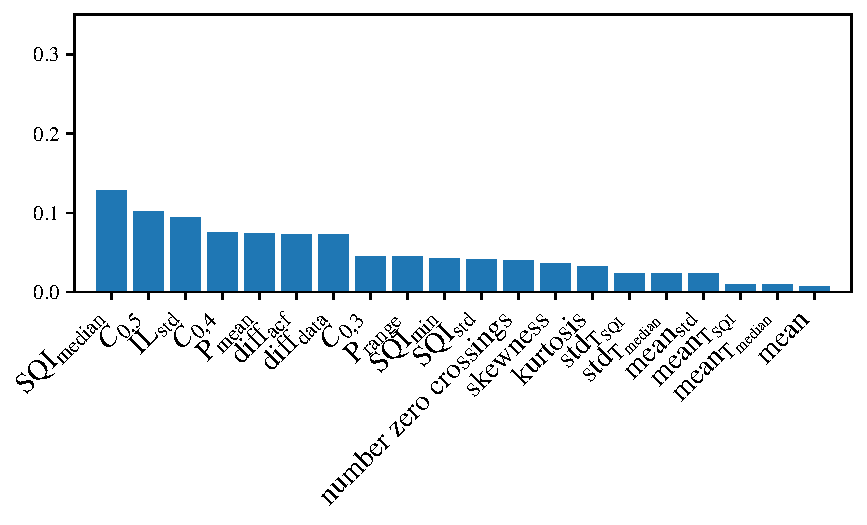
\includegraphics[width=\textwidth]{pic/rf-clf-reduced-importances.pdf}
 			\caption{\ac{RF}-Klassifikator}
 		\end{subfigure}
 	\caption{Vergleich der Wichtigkeit der Merkmale zwischen \ac{RF}-Klassifikator und \ac{XGB}-Klassifikator}
 	\label{fig:importances-comparison-rf-xgb-clf}
 \end{figure}

Betrachtet man die Wichtigkeit der Merkmale der Regressionsmodelle, gibt es kein einzelnes herausstechendes Merkmal. Auch die Wichtigkeit der einzelnen Merkmale ist, wie in Abbildung \ref{fig:importances-comparison-rf-xgb-regr} zu sehen, ähnlich verteilt.

 \begin{figure}[h]
 	\centering
		\begin{subfigure}{.495\textwidth}
			\centering
 			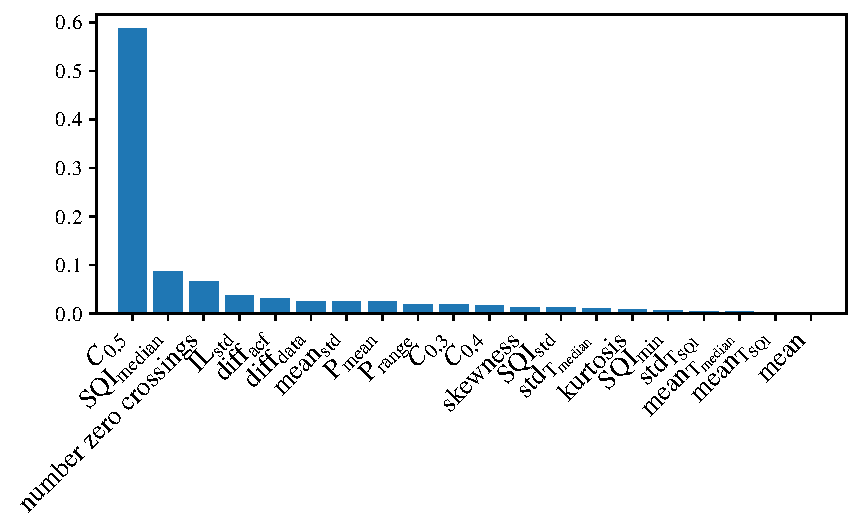
\includegraphics[width=\textwidth]{pic/xgb-regr-reduced-importances.pdf}
 			\caption{\ac{XGB}-Regressor}
 		\end{subfigure}
    	\begin{subfigure}{.495\textwidth}
    		\centering
 			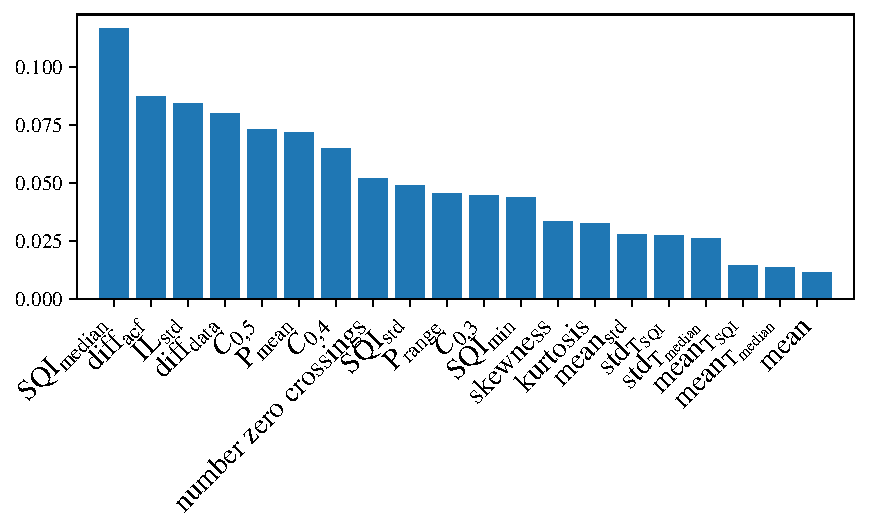
\includegraphics[width=\textwidth]{pic/rf-regr-reduced-importances.pdf}
 			\caption{\ac{RF}-Regressor}
 		\end{subfigure}
 	\caption{Vergleich der Wichtigkeit der Merkmale zwischen \ac{RF}-Regressor und \ac{XGB}-Regressor}
 	\label{fig:importances-comparison-rf-xgb-regr}
 \end{figure}

	
	\begin{itemize}
		\item Feature Importance aller plotten, jeweils reduziert und alle
		\item Vergleichen
		\item Modelle untereinander vergleichen
		\item recursive feature elminination
	\end{itemize}
	
	\section{Evaluation der Merkmale}

	\section{Einfluss der Segmentlänge}

	\section{Einfluss des Schwellwertes der Annotation}